
\subgroup{4}{Rob Ruigrok}

\paragraph{Description}
This chapter will cover the derivation of the dynamics of a heavy chain with uniform density $\rho$, length $L$ and a point mass on the end with mass $m$. The top of the chain will be suspended on a rolling trolley, where the lateral speed can be controlled. First, we will derive the dynamics, and later go into more detail on the "flatness" of the system and several control inputs.

\paragraph{Model}

An overview of the system is provided in figure \ref{fig:heavychainoverview}. Let $x$ be coordinate along the length of the chain, where the chain is attached to the trolley at $x=L$. The lateral displacement of the chain is denoted by $y(x,t)$. The problem can be made more complex by adding a point mass $m$ to the end of the chain.

\begin{figure}[h]
\label{fig:heavychainoverview}
\centering
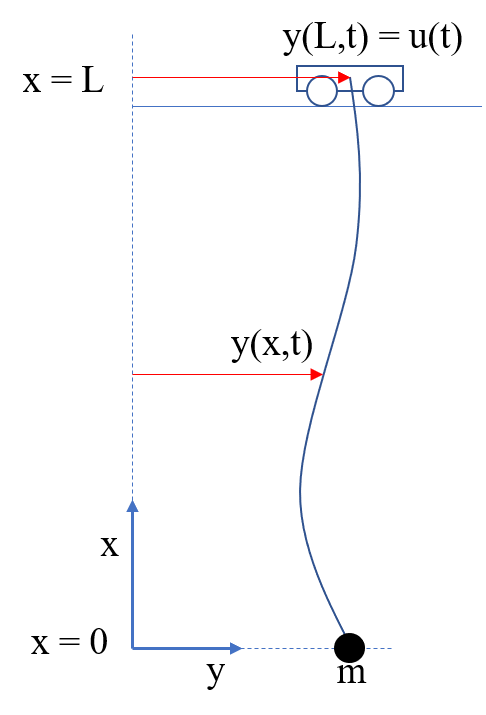
\includegraphics[width = 4cm]{Overview.png}
\end{figure}

The derivation of the dynamics goes largely the same as the derivation of the vibrating spring. Here, however, the tension in the chain will be depending on $x$, and there will now be different boundary conditions linked to the trolley at the top and the attached mass at the bottom. Figure \ref{fig:heavychaindx} illustrates the forces acting on a finite chain element of length $dx$, which is the basis in the derivation of the PDE.\newline

\begin{figure}[h]
\label{fig:heavychaindx}
\centering
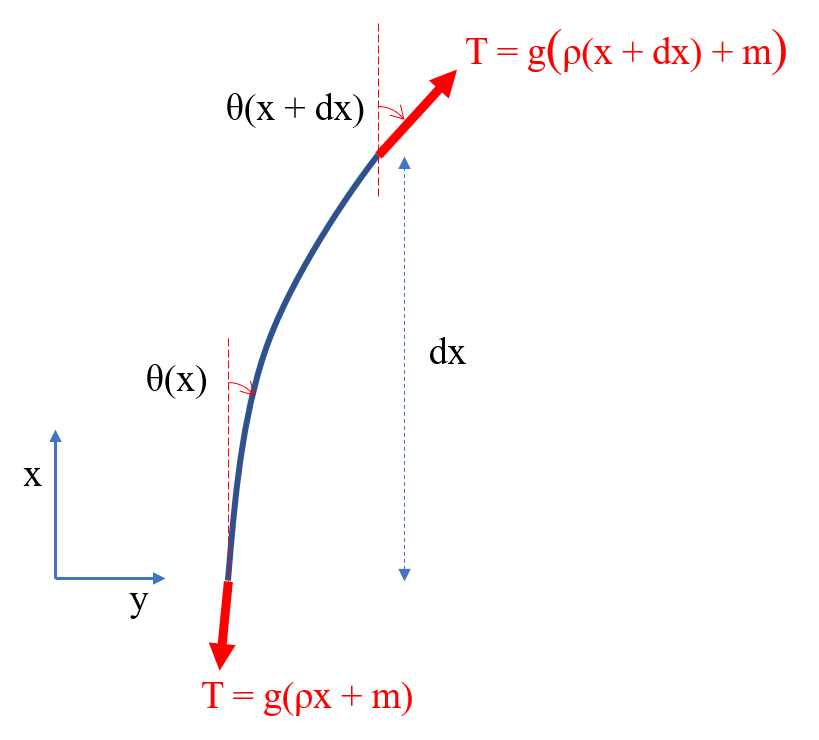
\includegraphics[width = 5cm]{SmallElement.png}
\end{figure}

We start with defining the tension in the chain as a function of $x$:

\begin{equation}
\label{eq:chaintension}
T = (m + x\rho)g
\end{equation}

To analyze the dynamics, we are interested of the lateral component of this tension. When examining an infinitesimal chain element of length $\Delta x$, we are interested in the net lateral force. Instead of defining the force on both sides of element $\Delta x$, we here determining the difference by using a first order Taylor approximation, together with a small angle approximation:

\begin{equation}
\label{eq:chainapprox}
sin(\theta)T \approx tan(\theta)T = \frac{\partial y}{\partial x}T
\end{equation}

\begin{equation}
\label{eq:chainforce}
\Delta F \approx F_x \Delta x = \big[\frac{\partial y}{\partial x}T\big]_x \Delta x
\end{equation}

The lateral motion of an infinitesimal chain element can now be described with Newtons second law of motion, $F = ma$, for which the net force is defined in equation \ref{eq:chainforce}. The mass of the chain element is $\rho \Delta x$, and the acceleration is $\frac{\partial^2 y}{\partial t^2}$

\begin{equation}
\begin{aligned}
    F &= ma \\
    \big[\frac{\partial y}{\partial x}T\big]_x \Delta x &= \rho \Delta x \frac{\partial^2 y}{\partial t^2} \\
    \big[\frac{\partial y}{\partial x} (m + x\rho)g \big]_x &= \rho \frac{\partial^2 y}{\partial t^2}
\end{aligned}
\end{equation}

When there is no mass suspended to end of the chain, the dynamics can be further written out:

\begin{eqnarray}
\label{eq:chainPDE}
    \big[\frac{\partial y}{\partial x} x \rho g \big]_x &=& \rho \frac{\partial^2 y}{\partial t^2} \\
    g \big[\frac{\partial y}{\partial x} x \big]_x &=& \frac{\partial^2 y}{\partial t^2} \\
    g \big[x \frac{\partial^2 y}{\partial x^2} + \frac{\partial y}{\partial x} \big] &=& \frac{\partial^2 y}{\partial t^2}
\end{eqnarray}
with boundary condition: $y(L,t) = u(t) $.


\paragraph{Solving the PDE}
\bigskip
\emph{\textbf{TODO: move part of it to control section
}}\bigskip

It is difficult to directly find a solution for the partial differential equation in equation~5\ref{eq:chainPDE}). For this particular problem, we assume that we know that we can rewrite to a Bessel function. Bessel functions are mainly used to describe wave propagation, and have the following format, where $\alpha$ denotes the order of the Bessel function:

\begin{equation}
\label{eq:Bessels}
x^2\frac{d^2 y}{dx^2} + x\frac{dy}{dx} + (x^2 - \alpha^2)y = 0
\end{equation}

In order to make the formulation in equation \ref{eq:chainPDE} fit this a zero-order Bessel function, we have to do certain changes of variables and convert the problem to the Laplace domain. In the Laplace domain, we can find solutions for our type of Bessel function, after which we need to transform it back to the time domain and reverse the variable changes. \newline

\paragraph{Step 1: substitution}

First step, do a substitution with $p = 2\sqrt{\frac{x}{g}}$. This will change the dependency from y(x,t) to y(p,t). Use the chain rule and find fill out the new values:

\begin{equation}
\label{eq:ChainRule}
\begin{aligned}
\frac{\partial p}{\partial x} &= \frac{1}{g}\bigg(\frac{x}{g}\bigg)^{-\frac{1}{2}} = \frac{1}{g\sqrt{\frac{x}{g}}} = \frac{2}{gp}\\
\frac{\partial y}{\partial x} &=  \frac{\partial y}{\partial p} \frac{\partial p}{\partial x} + \frac{\partial y}{\partial t} \cancelto{0}{\frac{\partial t}{\partial x}} = \frac{\partial y}{\partial p} \frac{2}{gp}
\end{aligned}
\end{equation}

When we fill everything out in the left part of equation \ref{eq:chainPDE}, we get the following expression:

\begin{equation}
\label{eq:chaincombination1}
\begin{aligned}
g \frac{\partial}{\partial x}\big[\frac{\partial y}{\partial x} x \big] &= g \frac{\partial}{\partial x}\big[\frac{\partial y}{\partial p} \frac{2}{gp} \frac{1}{4}gp^2 \big] = g \frac{\partial}{\partial x}\big[\frac{\partial y}{\partial p} \frac{p}{2} \big] \\
&= g \frac{\partial}{\partial p}\big[\frac{\partial y}{\partial p} \frac{p}{2} \big]\frac{\partial p}{\partial x} = g \big[\frac{\partial^2 y}{\partial p^2} \frac{p}{2} + \frac{1}{2} \frac{\partial y}{\partial p}\big] \frac{2}{gp} \\
&= \frac{\partial^2 y}{\partial p^2} + \frac{1}{p} \frac{\partial y}{\partial p}
\end{aligned}
\end{equation}

So the total equation can be written as:
\begin{eqnarray}
\label{eq:chaincombination2}
 g \big[\frac{\partial y}{\partial x} x \big]_x - \frac{\partial^2 y}{\partial t^2} &=& 0 \\
  \frac{\partial^2 y}{\partial p^2} + \frac{1}{p} \frac{\partial y}{\partial p} - \frac{\partial^2 y}{\partial t^2} &=& 0 \\
 p \frac{\partial^2 y}{\partial p^2} +
  \frac{\partial y}{\partial p} - p \frac{\partial^2 y}{\partial t^2} &=& 0
\end{eqnarray}

\paragraph{Step 2: transform to Laplace domain}

When converting the from the time domain, we use the following notation:
\begin{center}
$y(x,t) \xrightarrow{\mathcal{L}} Y(x,s)$
\end{center}
Further, to get the Laplace transform in the desired format, we require that the systems is initially \textit{at rest}, which means that $y(x,0)=0$ and $\dot{y}(x,0)=0$.

\begin{equation}
\label{eq:heavychainlaplace}
\begin{aligned}
 p \frac{\partial^2 y(x,t)}{\partial p^2} +
  \frac{\partial (x,t)}{\partial p} - p \frac{\partial^2 y(x,t)}{\partial t^2} = 0 \\
  \xrightarrow{\mathcal{L}}
 p \frac{\partial^2 Y(x,s)}{\partial p^2} +
  \frac{\partial Y(x,s)}{\partial p} - p s^2 Y(x,s) = 0
\end{aligned}
\end{equation}

NEW CHANGE OF VARIABLES (did it myself on paper, still need to isert)\newline
Bessel function!


